\documentclass[12pt, oneside]{book}

% Include necessary packages
\usepackage[nottoc]{tocbibind}
\usepackage{amsmath}
\usepackage{amsfonts}
\usepackage{amssymb}
\usepackage{graphicx}
\usepackage{float}
\usepackage{amsthm}
\usepackage{hyperref}
\usepackage{cleveref}
\usepackage{caption}
\usepackage{subcaption}
\usepackage{enumitem}
\usepackage{appendix}
\usepackage{titlesec}
\usepackage{lipsum}
\usepackage{setspace}
\usepackage{geometry}
\usepackage{pdflscape}
\usepackage{pdfpages}
\usepackage{wrapfig}
\usepackage{fancyhdr}
\usepackage{etoolbox}
\usepackage{mathrsfs}
\usepackage{tikz}
\usepackage{tikz-cd}
\usepackage{pgfplots}
\pgfplotsset{compat=1.18}
\usepackage{pgfplotstable}
\usepackage{booktabs}
\usepackage{array}
\usepackage{multirow}
\usepackage{longtable}
\usepackage{listings}
\usepackage{color}
\usepackage{colortbl}
\usepackage{braket}
\usepackage{tikz}
\usepackage{quantikz}
\usepackage{circuitikz}
\usepackage{algorithm}
\usepackage{algpseudocode}
\usepackage{tcolorbox}

% Define colors
\definecolor{codegreen}{rgb}{0,0.6,0}
\definecolor{codegray}{rgb}{0.5,0.5,0.5}
\definecolor{codepurple}{rgb}{0.58,0,0.82}
\definecolor{backcolour}{rgb}{0.95,0.95,0.92}
\definecolor{darkgreen}{rgb}{0.0, 0.2, 0.13}
\definecolor{darkred}{rgb}{0.55, 0.0, 0.0}
\definecolor{darkblue}{rgb}{0.0, 0.0, 0.55}
\definecolor{darkpurple}{rgb}{0.5, 0.0, 0.5}
\definecolor{darkcyan}{rgb}{0.0, 0.55, 0.55}
\definecolor{darkgray}{rgb}{0.66, 0.66, 0.66}
\definecolor{lightgray}{rgb}{0.95, 0.95, 0.95}

% Define styles and environments
\lstdefinestyle{mystyle}{
    backgroundcolor=\color{backcolour},   
    commentstyle=\color{codegreen},
    keywordstyle=\color{magenta},
    numberstyle=\tiny\color{codegray},
    stringstyle=\color{codepurple},
    basicstyle=\footnotesize,
    breakatwhitespace=false,         
    breaklines=true,                 
    captionpos=b,                    
    keepspaces=true,                 
    numbers=left,                    
    numbersep=5pt,                  
    showspaces=false,                
    showstringspaces=false,
    showtabs=false,                  
    tabsize=2
}
\lstset{style=mystyle}

\newtcolorbox{importantnote}{
    colback=lightgray,
    colframe=darkgray,
    fonttitle=\bfseries,
    title=Important Note
}

\newtheorem{problem}{Problem}[section]
\newtheorem{theorem}{Theorem}[section]
\newtheorem{lemma}[theorem]{Lemma}
\newtheorem{corollary}[theorem]{Corollary}
\newtheorem{proposition}[theorem]{Proposition}
\newtheorem{axiom}{Axiom}[section]
\theoremstyle{definition}
\newtheorem{definition}{Definition}[section]
\theoremstyle{definition}
\newtheorem{example}{Example}[section]
\theoremstyle{remark}
\newtheorem*{remark}{Remark}

% Define \abstractname and \acknowledgementsname
\newcommand{\abstractname}{Abstract}
\newcommand{\acknowledgementsname}{Acknowledgements}

\newenvironment{abstract}{%
\clearpage
\null\vfill
\begin{center}%
    \bfseries \abstractname
\end{center}}%
{\vfill\null}

\newenvironment{Acknowledgements}{%
\clearpage
\null\vfill
\begin{center}%
    \bfseries \acknowledgementsname
\end{center}}%
{\vfill\null}

\begin{document}

\frontmatter

\title{\vspace{-3.0cm}Quantum Error Correction}  % Title
\author{Nihar Shah}  % Author name
\date{\today}  % Date
\maketitle  % Print the title page

\begin{center}
\vspace*{2cm}
\textbf{Quantum Error Correction}\\[1cm]
\textbf{Nihar Shah}\\[1cm]
Guide: Professor Phani Motamarri
\vfill

\includegraphics[width=0.3\textwidth]{images/IISc_Master_Seal_Black.jpg}\\[1cm]
\large \textit{Department of Computational and Data Science}\\
\large \textit{Indian Institute of Science}
\vfill
\end{center}

\frontmatter

\begin{abstract}
The following content consists of the work done by me as a part of my Master's Thesis at Indian
Institute of Science, Bengaluru. The work is done under the guidance of Prof. Phani Motamarri. 
This work includes notes made during the 1 year work from June 2024 to August 2025 and is based on the
lectures, papers, books, and other resources that I have referred to during the course of my work.
To a reader who is not at all familiar with Quantum Computing, this work will serve as a good starting point. 
I suggest starting with the Appendix to get a good grasp of the math used in the entire text. 
The work is divided into parts: The first part is the introduction to Quantum Computing, the second part is Quantum Linear Algebra, the third part is on Quantum Information Theory and at last the fourth part is on Quantum Error Correction. Along with the references, 
I have also included the code snippets that I have written during the course of my work. The references are included at the end of the document.
I hope that this text helps the reader to get a good grasp on Quantum Computing. Enjoy reading!
\end{abstract}

% Acknowledgements
\begin{Acknowledgements}
\addcontentsline{toc}{chapter}{Acknowledgements}
First and foremost, I would like to express my sincere gratitude to my advisor,
Professor Phani Motamarri, for the continuous support of my study and related, for
his patience, and immense knowledge.
His guidance helped me through the time of research and writing of this thesis.

Besides my advisor, I am also grateful to the faculty members and staff at the
Department of Computational and Data Science of Indian Institute of Science for
their assistance and support. Special thanks to MATRIX lab for providing a stimulating
and collaborative research environment.

Last but not the least, I would like to thank my family: my parents,
for supporting me spiritually throughout writing this thesis and my life in general.
\end{Acknowledgements}

\tableofcontents

% Start of the main content
\mainmatter



\chapter{Classical Error Correction}
Before going to Quantum Error correction we will just take a step back and look at the Classical Error correction in order to understand in general the ideas of error correction.

\section{Background and Motivation}
We now talk about the communication system Model. In Shanon's 1948 paper on ``A mathematical Theory of Communication" he introduced a schematic diagram for a general communication system as shown in figure \ref{fig:comm_model}. By communication system we will mean a system of the type indicated schematically in figure \ref{fig:comm_model}. It consists of essentially five parts:
\begin{figure}
    \centering
    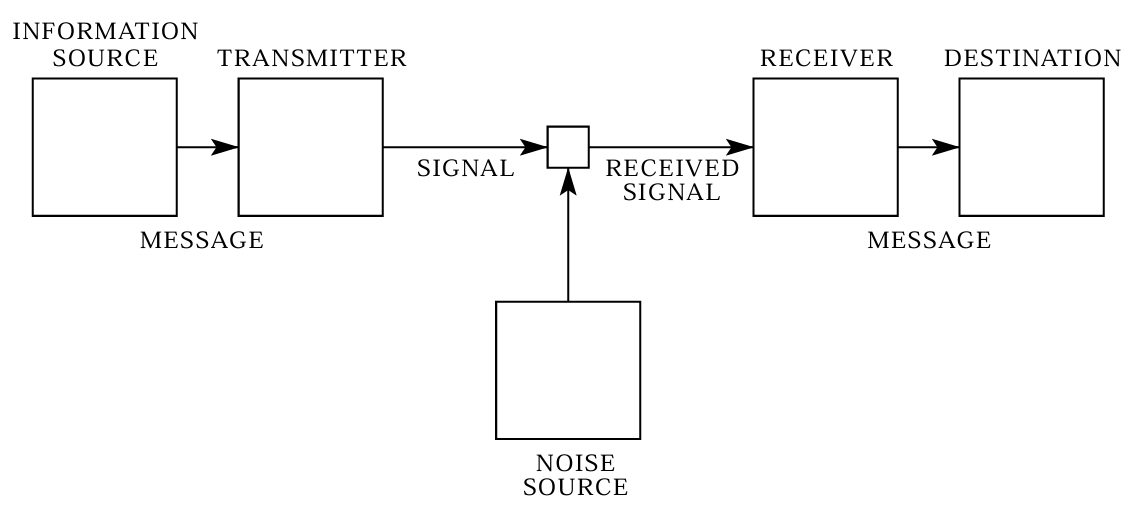
\includegraphics[width=0.75\linewidth]{../images/comm_model.png}
    \caption{Schematic diagram for a general communication system}
    \label{fig:comm_model}
\end{figure}
\begin{enumerate}
    \item An information source which produces a message or a sequence of messages to be communicated to the receiving terminal. The message may be of various types: (a) A sequence of letters as in a telegraph of teletype system; (b) A single function of time $f(t)$ as in radio or telephony; (c) A function of time and other variables as in black and white television - here the message may be though of as a function $f(x,y,t)$ of two space coordinates and time, the light intensity at point $(x,y)$ at time $t$ on a pickup tube plate; (d) Two or more functions of time, say $f(t),g(t),h(t)$ - this is the case in ``three-dimensional" sound transmission or if the system is intended to service several individual channels in multiplex; (e) Several functions of several variables - in color television the message consists of three function $f(x,y,t),g(x,y,t),h(x,y,t)$ defined in a three dimensional continuum - we may also think of these three functions as components of a vector filed define in the region- similarly, several black and white television sources would produce ``messages" consisting of a number of continuum of three variables; (f) Various combinations also occur, for example in television with an associated audio channel.
    \item A transmitter which operates on the message in some way to produce a signal suitable for transmission over the channel. In telephony this operation consists merely of changing sound pressure into a proportional electrical current. In telegraphy we have an encoding operation which produces a sequence of dots, dashes and spaces on the channel corresponding to the message. In a multiplex PCM system the different speech functions must be sampled, compressed, quantized and encoded, and finally interleaved properly to construct the signal. Vocoder systems, television and frequency modulation are other examples of complex operations applied to the message to obtain the signal.
    \item The channel is merely the medium used to transmit the signal from transmitter to receiver. It may be a pair of wires, a coaxial cable, a band of radio frequencies, a beam of light, etc.
    \item The receiver ordinarily performs the inverse operation of that done by the transmitted, reconstruction the message from the signal.
    \item The destination is the person (or thing) or whom the message is intended.
\end{enumerate}
 For analyzing, it is first necessary to represent the various elements involved as mathematical entities, suitably idealized from their physical counterparts. We may roughly classify communication systems into three main categories: discrete, continuous and mixed. By a discrete system we will mean one in which both the message and the signal are a sequence of discrete symbols. A typical case is telegraphy where the message is a sequence of letters and the signal a sequence of dots, dashes and spaces. A continuous system is one in which the message and signal are both treated as continuous functions, e.g., radio or television. A mixed system is one in which both discrete and continuous variables appear, e.g., PCM transmission of speech. 

We consider only the discrete case. This case has applications not only in communication theory, but also in the theory of computing machines, the design of telephone exchanges and other fields.

This naturally leads to the field of Coding theory. Coding is the representation using symbols, often 0s and 1s. What are the requirements for information transmission:
\begin{enumerate}
    \item Cost of transmission should be low
    \item Information should be transmitted reliably in the presence of channel noise
    \item Information should be transmitted securely in the presence of an adversary/eavesdropper
\end{enumerate}
The answer to each of these requirements is the following flavours of coding theory:
\begin{enumerate}
    \item Source Coding: Enables to compress message to save on transmission.
    \item Channel Coding: enables to send message reliably by introducing some mechanism to counter channel noise.
    \item Secrecy Coding (aka Cryptography): Enables to encrypt message to transmit message securely in presence of an adversary.
\end{enumerate}

Out of these three we will focus only on the first two parts i.e. Source Coding and Channel coding, which lead to Classical Error Correction. These two are closely related to Information theory. We assume that the Channel Noise follows a model known to both Information Source and Destination. This noise may be deterministic or random; if random, it follows a probabilistic model. The effect of noise is to introduce errors in the transmitted message and thus, the goal of channel coding is to reduce or eliminate the effects of channel noise.

Say Alice wishes to communicate with Bob a message made up of discrete symbols (0s and 1s). We will then use Source and Channel Coding to transmit the message. For the purpose of these notes, we ignore Secrecy coding aka Cryptography as Quantum Cryptography is in itself an entire field. We ignore the requirement of information to be transmitted securely in the presence of an adversary/eavesdropper. We wish to transmit the information at low cost and reliably in the presence of channel noise which can be achieved through source coding and Channel coding. There are three types of channel codes:
\begin{enumerate}
    \item \textbf{Error-Detecting Codes:} Allows Bob to detect errors in received message which is useful in random noise situations.
    \item \textbf{Error-Correcting Codes:} Allows Bob to correct errors in received message which is useful in random noise situations.
    \item \textbf{Constrained Codes:} Alice encodes the message in such a way as to prevent errors from corrupting the message which is useful in deterministic noise situations.
\end{enumerate}
\begin{importantnote}
    All coding schemes work by adding redundancy to the message to compensate for errors i.e more symbols are transmitted than are in the original message.
\end{importantnote}

\section{Error-Detecting Code}
Consider the following Error Detecting Code
\begin{figure}[h]
    \centering
    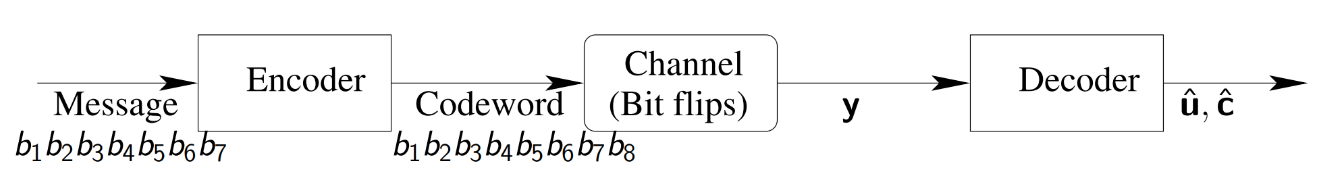
\includegraphics[width=0.75\linewidth]{../images/error-dect.png}
    \caption{A simple Error-Detecting Code}
    \label{fig:err-det}
\end{figure}
We wish to encode a message made up of a 7-bit binary sequence ($b_1,b_2,b_3,b_4,b_5,b_6,b_7$). As shown in figure \ref{fig:err-det} the encode adds 8th bit, called a parity bit, $b_8$, so that, $(b_1,b_2,\ldots,b_8$) contains an even number of 1s. Thus, the encode encodes the $7$ bit message to an $8$ bit message by adding a parity bit which is $1$ if there are an odd number of $1$ in the $7$-bit message and $0$ if there are an even bit of $1s$ in the message. Mathematically, we can write the foolwoing 
\[
\sum_{i=1}^{8} b_i=0 (\text{mod }2)
\]
Note that the addition is done in modulo $2$. The Channel noise model here is assume to randomly flip bits from $0\rightarrow 1$ and $1\rightarrow 0$. We now define Rate.

\begin{definition}
    \textbf{Rate:} The number of message bits per coded bits.
\end{definition}
For example, here the rate is $7/8$ because we have $7$ message bits and the codeword after encoding is of $8$ bits. Now consider the following example for a simple error-detecting code:
\begin{figure}[h]
    \centering
    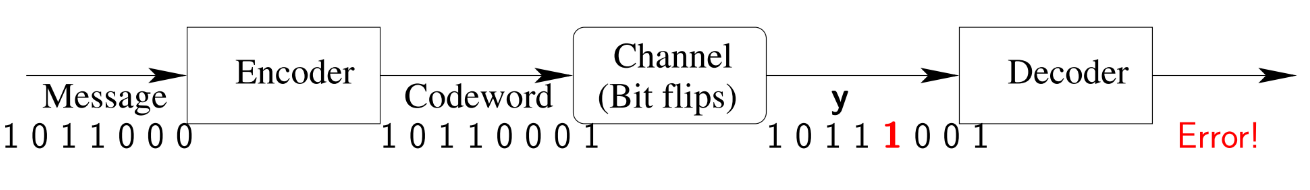
\includegraphics[width=0.75\linewidth]{../images/err-det-exa.png}
    \caption{Error Detecting Code example}
    \label{fig:err-exam}
\end{figure}
We define the decoder as follows
\[
c = \begin{cases} 
$y$, & \text{if $y$ has even parity}\\
$ERROR$, &\text{if $y$ has odd parity} 
\end{cases}
\]
We now define error to occur when the received message is not the same as the intended message. In this case we assume the channel model that random bit flip of $0$ to $1$ or $1$ to $0$ may occur. Now there are various errors that can occur. Note that this code detects an odd number of errors. That is, if odd number of $0s$ changes to $1s$ or odd number of $1s$ changes to $0s$. The code can detect an error has occurred but it cannot detect where error has occurred. Also, it cannot detect an error in cases such as when a $0$ flips to $1$ and a $1$ flips to $0$ maintaining the parity but the message changes. In this case, it cannot detect an error. Only in the case when it the cases when the parity changes to odd is it can detect error. In all other errors, when the parity remains even it assumes that the codeword is correct (even though there could be cases where the flips occur in such a way that the parity did not change but the message did. For example, in the above case when the codeword $10110001$ changes to $10101001$, note that the parity is still even but clearly the message has changed). Thus, the decoder designed above can detect error only when $y$ has odd parity, in all other cases, it assumes that no error has occurred. When the decoded detects an error, it sends a message to encoder to resend the message.

These kind of Error-detection codes has applications in Computer network communication protocols, International Standard Book Numbers(ISBN). Network protocols such as TCP/IP use error-detecting codes extensively to determine if data packets sent across a network have been corrupted or not. The usual remedy for receipt of a corrupted data packet is to request retransmission. ISBN-10 numbers have 10 digits and are of the form x-xxx-xxxxx-x. The first nine digits in an ISBN record information about the country book: country, published, title, and edition. The tenth digit is a check digit.


\subsection{Memoryless Binary symmetric channels}
Say Alice wants to send a $k$-bit message to Bob. The message is to be transmitted across a memoryless binary Symmetric Channel. Each bit transmitted across the channel gets flipped with probability $p$, independently of other bits. Say $k=10000$ and $p=0.001$. Say the transmission is uncoded, thus, the rate $=1$. The probability that the entire $k$-bit message is recovered by Bob:
\[
P_C=(1-p)^k=0.000045
\]
for $k=10000$ and $p=0.001$.

For an example of a situation in which the chances of making an error can be decreased using a repetition code, suppose that our goal is to communicate a single bit to a hypothetical receiver, and we're able to transmit bits through a so-called binary symmetric channel, which flips each bit sent through it independently with some probability $p$/ That is, with probability $1-p$ the receiver gets whatever bit was sent through the channel, bit with probability $p$ the bit flips and the receiver gets the opposite bit value.
\subsection{Classical repetition codes}
We'll begin the lesson with classical repetition codes, which form the basis for the 9-qubit Shor code.


\subsubsection{Encoding and Decoding}
Repetition codes are extremely basic examples of error correcting codes. The idea is that we can protect bits against error by simply repeating each bit some fixed number of times. In particular, let's first consider the $3$-bit repetition code. Here we encode one bit into three by repeating the bit three times, so $0$ is encoded as $000$ and $1$ is encoded as $111$.

If nothing goes wrong we can obviously distinguish the two possibilities for the original bit from their encodings. The point is that if there was an error and one of the three bits flipped, meaning that a $0$ changes into a $1$ or a $1$ changes to $0$, then we can still figure out what the original bits was by determining which one of the two binary values appear twice. Equivalently, we can decode by computing the majority value (i.e., the binary value that appears most frequently)
\[
abc \rightarrow majority(a,b,c)
\]
Of course, if $2$ or $3$ bits of the encoding flip, then the decoding won't work properly and the wrong bit will be recovered, but if at most $1$ of the $3$ bits flips, the decoding will be correct. Thus, this code can correct single errors and the rate is $\frac{1}{3}$. This is a typical property of error correcting codes: they may allow for the correction of errors, but only if there aren't too many of them.

So, if we choose  not to use the $3$ bit repetition code, and simply send whatever bit we have in mind through the channel, the receiver therefore receives the wrong bit with probability $p$. On the other hand, if we first encode the bit we want to send using the $3$ bit repetition code, and then send each of the three bits of the encoding through the channel, then each of them flips independently with probability $p$. The changes of a bit-flip are now greater because there are now three bits that might flip rather than one - but if at most one bit flips then the receiver will decode correctly. So, an error persists after decoding only if two or more of the bits flip during transmission.

The probability that two bits flip during the transmission is $3p^2(1-p)$, which is $p^2(1-p)$ for each of the three choices for the bit that doesn't flip, while the probability that all the three bits flip is $p^3$. The total probability of two or three bit flips is therefore
\[
1-P_{b,C}=3p^2(1-p) + p^3 = 3p^2-2p^3
\]
Thus, the probability that an entire $k$-bit message is decoded correctly is
\[
P_C=(P_{b,c})^k\approx 0.97
\]
for $k=10000$ and $p=0.001$. Note that $30000$ coded bits are actually transmitted since the rate is $\frac{1}{3}$.

For values of $p$ smaller than one-half this results in a decrease in the probability that the receiver ends up with the wrong bit. There will still be a chance of an error in this case, bit the code decreases the likelihood (For values of $p$ greater than one-half, on the other hand, the code actually increases the likelihood that the receiver gets the wrong bit.) See figure \ref{fig:errrprob}.
\begin{figure}[ht]
    \centering
    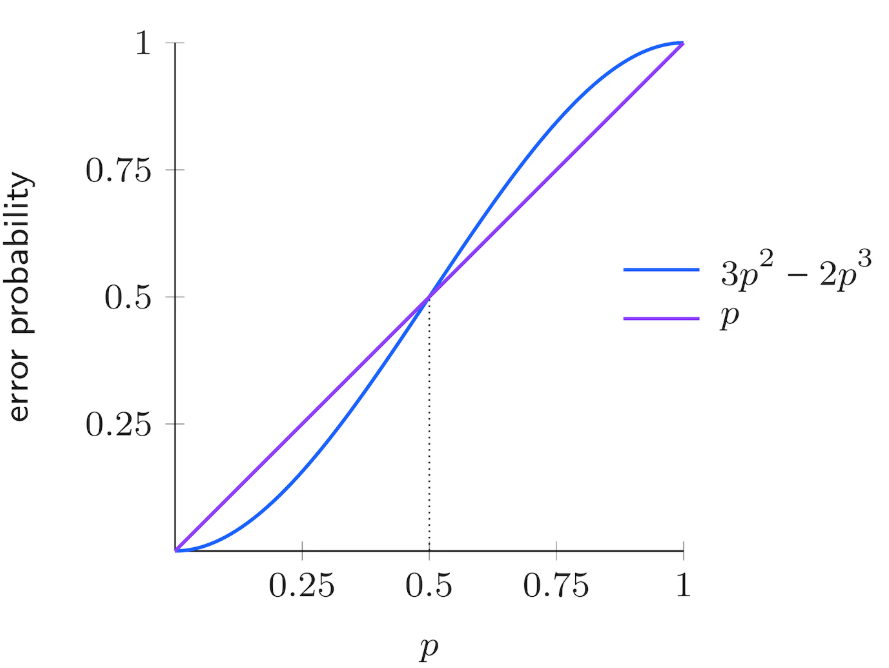
\includegraphics[width=0.75\linewidth]{../images/grapherr.png}
    \caption{Error probability vs p}
    \label{fig:errrprob}
\end{figure}

\section{Error-Correcting Code}
\subsection{The Length-$7$ Hamming Code}
This code was discovered by Richard hamming in 1950. It encodes a $4$ bit message into a $7$-bit codeword:
\[
u_1u_2u_3U-4\rightarrow u_1u_2u_3u_4p_1p_2p_3
\]
where $u_i;i=1,2,3$ are information bits and $p_i;i=1,2,3$ are parity bits. Thus, the rate for the code is $\frac{4}{7}$. Consider the following figure \ref{fig:7bithamcode}. For each choice of $(u_1,u_2,u_3,u_4)$, there is a unique choice of $(p_1,p_2,p_3)$ that makes each circle have even number of $1s$.

\begin{figure}
    \centering
    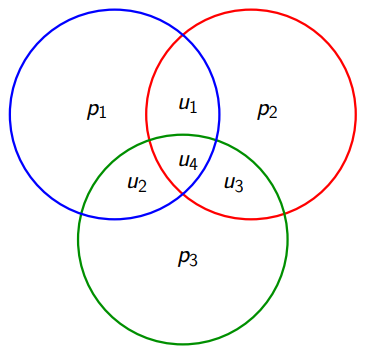
\includegraphics[width=0.5\linewidth]{../images/7bithamm.png}
    \caption{Length-$7$ Hamming Code}
    \label{fig:7bithamcode}
\end{figure}

This can be written as follows in the form of equations:
\begin{align*}
    u_1+u_2+u_4+p_1 &\equiv 0 \quad \text{(mod 2)}\\
    u_1+u_3+u_3+p_2 &\equiv 0 \quad \text{(mod 2)}\\
    u_2+u_2+u_3+p_3 &\equiv 0 \quad \text{(mod 2)}
\end{align*}
For example, if the information bits $u_1=1,u_2=0,u_3=0$ then the codeword in the Hamming code will be $1000110$ where $p_1=1,p_2=0,p_3=0$.

Now, consider the following Decoder for Hamming code. Let Alice send information $(u_1,u_2,u_3,u_4)$ which gets encoded to $(u_1,u_2,u_3,u_4,p_1,p_2,p_3)$ in the encoder. Thus, the codeword is $(u_1,u_2,u_3,u_4,p_1,p_2,p_3)$. We assume the channel noise model that flips bits at random $(o\rightarrow 1 , 1\rightarrow 0$. Suppose that Alice sends $1000110$, but Bob receives $1100110$. Note that the second bit is flipped from $0$ to $1$. In order to decode we follow the following procedure. Consider the figure \ref{fig:7bithamcodeexa}. We use the following rules to decode. Thus, decoder (Bob) uses the following decoding model:
\begin{enumerate}
    \item Identify circles with wrong parity.
    \item Flip bit common to those circles only.
\end{enumerate}
\begin{figure}
    \centering
    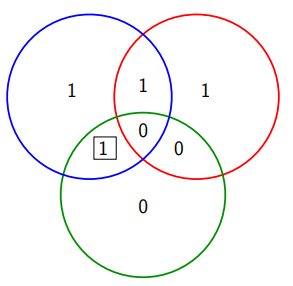
\includegraphics[width=0.5\linewidth]{../images/7bithamcodeex.png}
    \caption{$7$-bit Hamming Code Example}
    \label{fig:7bithamcodeexa}
\end{figure}
We can clearly, see that circles blue and green are the ones with wrong parity and thus, the bit common only to these two circles is as shown in figure \ref{fig:7bithamcodeexa}. Thus, we flip that $1$ to $0$ and we now have all the circles satisfying the parity. Hence, we have corrected the code and recovered the original message. Like in the case of $3$-bit repetition codes based on majority, we can only correct single errors. If there are errors in more than one bit then they cannot be corrected. But there is an interesting case, consider the case when there are errors in two bits. In that case, we can may not be able to correct the errors but we can still detect errors and thus, can request for retransmission. In the case when the errors are in more than $2$ bits we are may not be able to even detect nor correct an error that has occurred.

Now consider we wish to transmit a $k$-bit message, we first divide the message into $4$-bit blocks, encode using a $7$-bit codeword, and transmit. Thus, $k/4$ codewords i.re. $7k/4$ coded bits are transmitted. Recall that we can correct one-bit errors. Thus, the probability that the codeword is transmitted correctly or with at most one bit error is
\[
Pr[\text{at most one of the $7$ bits is flipped}]=(1-p)^7 + 7p(1-p)^6
\]
Hence, the probability that the entire $k$-bit message is recovered correctly by Bob is
\[
P_C=[(1-p)^7+7p(1-p)^6]^{k/4}\approx 0.95
\]
for $k=10000$ and $p=0.001$ where we transmitted $7k/4=7\times 10000/4=17500$ coded bits.

\begin{importantnote}
    \textbf{Shannon's Noisy Channel Coding Theorem}\\
    We assume the Channel model to be memoryless binary symmetric channel with crossover probability $p$. Then the Channel Capacity of the Binary Symmetric Channel is given as:
    \[
    C(p)=1+p\log_2 p+(1-p)\log_2(1-p)
    \]
    \begin{theorem}
        If rate $R<C(p)$ and $k$ is sufficiently large, there exists a code which can encode $k$ message bits into $n=k/R$ coded bits to be transmitted across the channel, such that a decoder at the channel output can recover all $k$ message bits correctly with probability close to $1$.
    \end{theorem}
    Note that $C(0.001)\approx 0.9886$. This means that to ensure that a $10000$-bit message can be recovered correctly with probability close to $1$, it should be enough to transmit about $10000/0.9886 \approx 10150$ coded bits.
\end{importantnote}

The goal of coding theory is to design coding schemes that can approach Shannon's performance guarantees, while still being relatively easy to implement in practice. We are interested in low complexity, and good error-correction capability.

\section{Linear Codes}
Let $\mathbb{F}_q$ denote a finite field of size $q$. For concreteness, take $q=2$, i.e. $\mathbb{F}_2$ is the binary field $\{0,1\}$ with modulo-2 arithmetic. We will denote $\mathbb{F}_q^n = \{(x_1,x_2,\ldots,x_n): x_i \in \mathbb{F}_q\}$. Clearly, the number of elements, $|\mathbb{F}_q^n|=|\mathbb{F}_q|^n =q^n$.

\begin{definition}
    A linear code $\mathcal{C}$ of block length $n$ over $\mathbb{F}_q$ is a linear subspace of $\mathbb{F}_q^n$. For each pair $\mathbf{c_1},\mathbf{c_2}\in \mathcal{C}$ and for any $\alpha_1,\alpha_2 \in \mathbb{F}_q$, we also have $\alpha_1\mathbf{c_1}+\alpha_2\mathbf{c_2}\in\mathcal{C}$.
\end{definition}
The dimension of a code $\mathcal{C}$ is the dimension of $\mathcal{C}$ as a linear subspace of $\mathbb{F}_q^n$ over $\mathbb{F}_q$; denoted by $dim(\mathcal{C})$ or $dim_{\mathbb{F}_q}(\mathcal{C})$.

A $[n,k]$ linear code is a linear code of blocklength $n$ and dimension $k$.

\begin{proposition}
An $[n,k]$ linear code $\mathcal{C}$ over $\mathbb{F}_q$ has $q^k$ codewords.
\end{proposition}
\begin{proof}
    An $[n,k]$ linear code $\mathcal{C}$ can be uniquely expressed as a linear combination
    \[
    \mathbf{c}=\alpha_1\mathbf{c_1}+\alpha_2\mathbf{c_2}+\ldots+\alpha_k\mathbf{c_k}
    \]
    with $\alpha_j\in\mathbb{F}_q \forall j$. Thus, there is a $1-1$ correspondence between codewords $\mathbf{c}\in\mathcal{C}$ and $k$-tuples of coefficients $(\alpha_1,\ldots,\alpha_k)\in\mathbb{F}_q$. Hence $|\mathcal{C}|=|\mathbb{F}_q^k|=q^k$.
\end{proof}
The rate of an $[n,k]$ linear code over $\mathbb{F}_q$ is
\[
R=\frac{k}{n}
\]

\begin{example}
    The repetition code over $\mathbb{F}_2:\{00\ldots0,11\ldots1\}$. This is a linear code over $\mathbb{F}_2$ with block length $n$ and dimension $1$. In other words, this is an $[n,1]$ binary linear code.
\end{example}

\begin{example}
    The single parity-check code over $\mathbb{F}_2$:
    \[
    \mathcal{C}=\{x_1x_2\ldots x_n: x_1+x_2+\ldots+x_n\equiv 0 \text{ (mod 2)}\}=nullspace(H)
    \]
    where $H=\begin{bmatrix}
        1 &1 & \ldots & 1 
    \end{bmatrix}$. By the rank-nullity theorem,
    \[
    dim(\mathcal{C})=n-rank(H)=n-1
    \]
    Thus, $\mathcal{C}$ is an $[n,n-1]$ binary linear code.
\end{example}

\begin{example}
    \textbf{(The Length-7 Hamming code)} Recall that a binary word $x_1,x_2,\ldots,x_7$ is in the Hamming code iff
    \begin{align*}
        x_1+x_2+x_4+x_5 &\equiv 0\quad \text{(mod 2)}\\
        x_1+x_3+x_4+x_6 &\equiv 0\quad \text{(mod 2)}\\
        x_2+x_3+x_4+x_7 &\equiv 0\quad \text{(mod 2)}
    \end{align*}
    rewriting this equations in matrix form (over $\mathbb{F}_2$) as
    \[
    \begin{bmatrix}
        1 &1 & 0 & 1 & 1 & 0 & 0 \\
        1 & 0 & 1 & 1 & 0 & 1 & 0 \\
        0 & 1 & 1 & 1 & 0 & 0 & 1
    \end{bmatrix}
    \begin{bmatrix}
        x_1 \\ x_2 \\ x_3 \\ x_4 \\ x_5 \\x_6 \\ x_7 
    \end{bmatrix}
    =\begin{bmatrix} 0 \\ 0 \\ 0 \end{bmatrix}
    \]
    
The binary word $x_1x_2x_3x_4x_5x_5x_7$ is the Hamming code $\mathcal{C}$ iff the above equations are satisfied.

In other words, the Hamming code $\mathcal{C}$ is equal to nullspace $\mathbb{F}_2(H)$. Consequently, by rank-nullity theorem, $dim(\mathcal{C})=n-rank_{\mathbb{F}_2}(H)=7-3=4$. Thus, $\mathcal{C}$ is a $[7,4]$ linear code.
\end{example}

\subsection{Minimum Distance}
Let $\mathbf{c}=(c_1,c_2,\ldots,c_n)$ and $\mathbf{c'}\in(c_1',c_2',\ldots,c_n')$ be words in $\mathbb{F}^n$. 
\begin{definition}
    \textbf{(Hamming Distance)} The Hamming distance between $\mathbf{c}$ and $\mathbf{c'}$ is defined to be
\[
d(\mathbf{c},\mathbf{c'})=|\{i:c_i\neq c_i'\}|
\]
\end{definition}
\begin{definition}
    \textbf{(Hamming Weight)} The Hamming weight of $\mathbf{c}$ is defined to be
\[
w(\mathbf{c})=d(\mathbf{c},\mathbf{0})=|\{i:c_i\neq 0\}|
\]
\end{definition}

\begin{definition}
  \textbf{(Minimum distance)} The minimum distnace of a linear code $\mathcal{C}$ is
  \[
  d_{min}(\mathcal{C})=\min_{\mathbf{c},\mathbf{c'}\in\mathcal{C}:\mathbf{c}\neq \mathbf{c'}} d(\mathbf{c},\mathbf{c'})=\min_{\mathbf{c}\in\mathcal{C}:\mathbf{c}\neq \mathbf{0}}w(\mathbf{c})
  \]
  An $[n,k,d]$ linear code is an $[n,k]$ linear code with minimum distance $d$.
\end{definition}

\begin{example}
    The repetition code over $\mathbb{F}_2 :\{00\ldots0,11\ldots,1\}$ is a $[n,1,n]$ binary linear code.
\end{example}

\begin{example}
    The single parity-check code over $\mathbb{F}_2$:
    \[
    \mathcal{C}=\{x_1x_2\ldots x_n:x_1+x_2+\ldots+x_n\equiv 0\quad \text{(mod 2)}\}
    \]
    Since there are no codewords of (odd) weight 1, and all binary words of (even) weight are in the code $dim(\mathcal{C})=2$. Thus, this is an $[n,n-1,2]$ binary linear code.
\end{example}

\begin{example}
    \textbf{(The Length-7 Hamming code)} A binary words $x_1x_2x_3x_4x_5x_6x_7$ is in the Hamming code $\mathcal{C}$ iff
    \[
    \begin{bmatrix}
        1 &1 & 0 & 1 & 1 & 0 & 0 \\
        1 & 0 & 1 & 1 & 0 & 1 & 0 \\
        0 & 1 & 1 & 1 & 0 & 0 & 1
    \end{bmatrix}
    \begin{bmatrix}
        x_1 \\ x_2 \\ x_3 \\ x_4 \\ x_5 \\x_6 \\ x_7 
    \end{bmatrix}
    =\begin{bmatrix} 0 \\ 0 \\ 0 \end{bmatrix}
    \]
    i.e. $Hx^T=\mathbf{0}$, we can simplify the above expression into
    \[
    x_1\begin{bmatrix} 1\\1\\0\end{bmatrix} + x_2\begin{bmatrix} 1\\0\\1\end{bmatrix}
    +x_3\begin{bmatrix}0 \\ 1 \\ 1 \end{bmatrix} + x_4\begin{bmatrix}
        1\\1\\1
    \end{bmatrix} + x_5 \begin{bmatrix} 1\\0\\0\end{bmatrix} +x_6\begin{bmatrix}0\\1\\0\end{bmatrix} +x_7\begin{bmatrix}0\\0\\1\end{bmatrix} =\begin{bmatrix} 0 \\ 0 \\ 0 \end{bmatrix}
    \]
    Now, note that $\mathcal{C}$ has no codewords of weight $1$, as no columns of $H$ is $\mathbf{0}$. $\mathcal{C}$ has no codewords of weight $2$, as no two columns of $H$ are identical. $\mathcal{C}$ does have codewords of weight $3$: e.g., the first three columns of $H$ sum to $\mathbf{0}$ over $\mathbb{F}_2$, so $1110000$ is in $\mathcal{C}$. Hence, $d_{min}(\mathcal{C})=3$. Thus, the Hamming code is a $[7,4,3]$ binary linear code.
\end{example}

Let $\mathcal{C}$ be a linear code of $\mathbb{F}$ with parity-check matrix $H$, i.e., $\mathcal{C}=nullspace_{\mathbb{F}}(H)$.

\begin{theorem}
    The minimum distance of $\mathcal{C}$ is equal to the smallest number of columns of $H$ that are linearly dependent over $\mathbb{F}$. Equivalently, $d_{min}(\mathcal{C})$ is the largest integer $d$ such that every collection of $d-1$ columns of $H$ is linearly dependent over $\mathbb{F}$.
\end{theorem}

If $\mathcal{C}=nullspace_{\mathbb{F}}(H)$, then $H$ is called a parity-check matrix for $\mathcal{C}$.

\subsection{Error Correction}
Given a length $n$ code $\mathcal{C}$. An error is an even of changing an entry in a codeword. A code words $\mathbf{c}\in\mathcal{C}$ is transmitted, and $\mathbf{y}\in\mathbb{F}^n$ is received. The number of errors that have occurred is $d(\mathbf{y},\mathbf{c})$.
\begin{definition}
    A code $\mathcal{C}$ is $t$-error-correcting if there exists a decoding map $ D:\mathbb{F}^n\rightarrow \mathcal{C}$ such that whenever $d(\mathbf{y},\mathbf{c})\leq t$, we have $\mathcal{D}(\mathbf{y})=c$.
\end{definition}

\begin{proposition}
    A $[n,k,d]$ code is $t$-error correction for $t<d/2$.
\end{proposition}
\begin{proof}
    A codeword $\mathbf{c}\in\mathcal{C}$ is transmitted, and $\mathbf{y}in\mathbb{F}^n$ is received. The number of errors that have occurred is $d(\mathbf{y},\mathbf{c})$. Decode $\mathbf{y}$ to closest codeword: $\hat{\mathbf{c}}=arg \min_{\mathbf{c'}\in\mathcal{C}}d(\mathbf{y},\mathbf{c'})$. If $d(\mathbf{y},\mathbf{c})<d/2$, then $\hat{\mathbf{c}}=\mathbf{c}$.
\end{proof}

\subsection{Erasures}
An erasures is an error whose location is known. Usualy represented by a `?' symbol:
\begin{figure}[h]
    \centering
    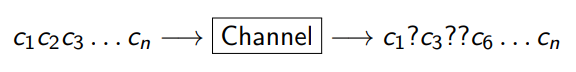
\includegraphics[width=0.5\linewidth]{../images/erasure.png}
    \caption{Erasure}
\end{figure}

\begin{proposition}
    Let $\mathcal{C}$ be an $[n,k,d]$ code over $\mathbb{F}$. There is a decode for $\mathcal{C}$ that corrects any occurrence of up to $d-1$ erasures.
\end{proposition}
\begin{proof}
    Let $\Phi=\mathbb{F}\cup \{?\}$. Consider the decoder defined for each $\mathbf{y}\in \Phi^n$ as
    \[
    \mathcal{D}(\mathbf{y})=\begin{cases}
        \mathbf{c} &\text{if $\mathbf{c}$ is the unique codeword that agrees with $\mathbf{y}$ on all unerased positions}\\
        ERROR &\text{otherwise}
    \end{cases}
    \]
    Suppose that $\mathbf{c}$ was transmitted and at most $d-1$ of its coordinates were erased. The received word $\mathbf{y}$ contains at most $d-1$ `?' symbols, and agrees with $\mathbf{c}$ on all the unerased positions. If there were another $\mathbf{c'}\in\mathcal{C}$ that also agreed with $\mathbb{y}$ on all the unerased positions, then $\mathbf{c}$ and $\mathbf{c'}$ could differ only in those positions where $\mathbf{y}$ has `?' symbols. Then, $d9\mathbf{c},\mathbf{c'}\leq d-1$, which contradicts $d_{min}(\mathcal{C})=d$. Thus, $\mathbf{c}$ is the unique codeword that agrees with $\mathbf{y}$ in all unerased coordinated, and hence $\mathcal{D}(\mathbf{y},\mathbf{c})$.
\end{proof}








\chapter{Quantum Noise and Quantum Error-Correcting Codes}


Quantum computation has the potential to enable efficient solution to computational tasks for which efficient classical algorithms are not known, and possibly don't exist. there are, however, very significant challenges that will need to be overcome before we can reliably implement the sorts of large-scale quantum computations we hope will one day be possible.

The heart of the matter is that quantum information is extremely fragile - you can literally ruin it just by looking at it. for this reason, to correctly operate, quantum computers need to isolate the quantum information they store from the environment around them to an extreme degree. But at the same time, quantum computers must provide the user with very precise control over this quantum information, including proper initialization, accurate and reliable unitary operations, and the ability to perform measurements so that the result of the computation can be obtained.

There's clearly some tension between these requirements, and in the early days of quantum computing some viewed that the fragility of quantum information, and its susceptibility to both inaccuracies and environmental noise, would ultimately make quantum computing impossible. today, there's little doubt that building an accurate and reliable large-scale quantum computer is a monumental challenge. But we have a key tool to help us in this endeavour that leads most people who are knowledgable about the field to be optimistic about large-scale quantum computing one day becoming a reality, and that tool is quantum error correction.

Next we will discuss quantum error correction, with a focus on the fundamentals. In this we'll take a first look at quantum error correction, including the very first quantum error correction code discovered - the 9 qubit shor code and we will also discuss a foundational concept in quantum error correction known as the discretization of errors.

\section{Repetition code for qubits}
The $3$ bit repetition code is a classical error-correcting code, but we can consider what happens if we try to use it to protect qubits against errors. As we'll see, it's not a very impressive quantum error correcting code: it actually makes some errors more likely. It is, however, the first step towards the Shor code, and it will also serve us well from a pedagological viewpoint.

\subsection{Encoding}
To be clear, when we refer to the $3$-bit repetition code being used for qubits, we have in mind an encoding of a qubit where standard basis states are repeated three times, so that single-qubit state vector is encoded as follows
\[
\alpha\ket{0}+\beta\ket{2}\rightarrow \alpha\ket{000}+\beta\ket{111}
\]
This encoding is easily implemented by the following quantum circuit in figure \ref{fig:3bitrepcirc} that makes use of two initialized workspace qubits and two controlled-NOT gates.
\begin{figure}[ht]
    \centering
    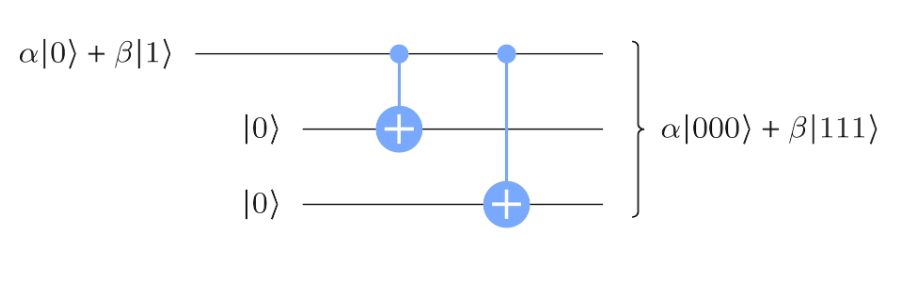
\includegraphics[width=0.75\linewidth]{../images/bitflipprep.png}
    \caption{3-bit repetition code circuit}
    \label{fig:3bitrepcirc}
\end{figure}
Notice in particular that this encoding is not the same as repeating the quantum state three times, as in a given qubit state vector being encoded as $\ket{\psi}\rightarrow \ket{\psi}\ket{\psi}\ket{\psi}$. Such an encoding cannot be implemented for an unknown quantum state $\ket{\psi}$ by the no cloning theorem.

\subsection{Bit-Flip error detection}
Now suppose that an error takes place after the encoding has been performed. In particular, let's suppose that an $X$ gate, or in other words a bit flip occurs on one of the qubits. For instance, if the middle qubit experiences a bit-flip, the state of the three qubits is transformed into this state:
\[
\alpha\ket{010}+\beta\ket{101}
\]
Of course this isn't the only sort of error that could occur - and it's also reasonable to question the assumption that an error takes the form of a perfect, unitary operation. We'll return to these issues in the last section of the lesson, and for now we can view an error of this form as being just one possibility (albeit a fundamentally important one) for an error.

We can see clearly from the mathematical expressing for the state above that the middle bit is the one that's different inside of each ket - but suppose that we had the three qubits in our possession and didn't know their state. If we suspected that a bit-flip may have occurred, one option to verify that a bit flipped would be to perform a standard basis measurement, which in the case at hand causes us to see $010$ or $101$ with probabilities $|\alpha|^2$ and $|\beta|^2$, respectively. In either case our conclusion would be that the middle bit flipped - but unfortunately the original quantum state $\alpha\ket{0}+\beta\ket{1}$ is now lost. This is the state we're trying to protect, so measuring the standard basis is an unsatisfactory option.

What we can do instead is to use the following quantum circuit, feeding the encoded state into the top three qubits. This circuit in figure \ref{fig:bitfliperr} non-destructively measures the parity of the standard basis states of the top two qubits as well as the bottom two qubits of the three-qubit encoding.
\begin{figure}[ht]
    \centering
    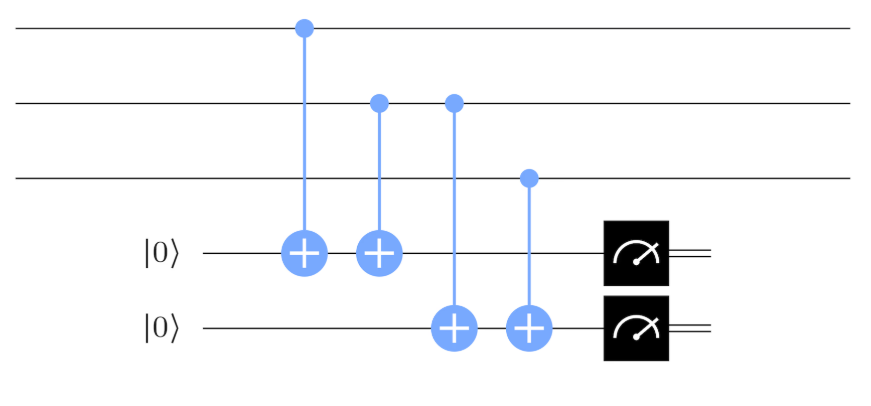
\includegraphics[width=1\linewidth]{../images/possbitflipcircs.png}
    \caption{Bit-Flip Error correction circuit}
    \label{fig:bitfliperr}
\end{figure}
Under the assumption that at most one bit flipped, one can easily deduce from the measurement outcomes the location of the bit flip (or the absence od one). In particular, as the following four circuit diagrams \ref{fig:possbitflip}, illustrate the measurement outcome $00$ indicates that no bit flip occurred, while the three other possibilities indicate which qubit experienced a bit flip.
\begin{figure}[ht]
    \centering
    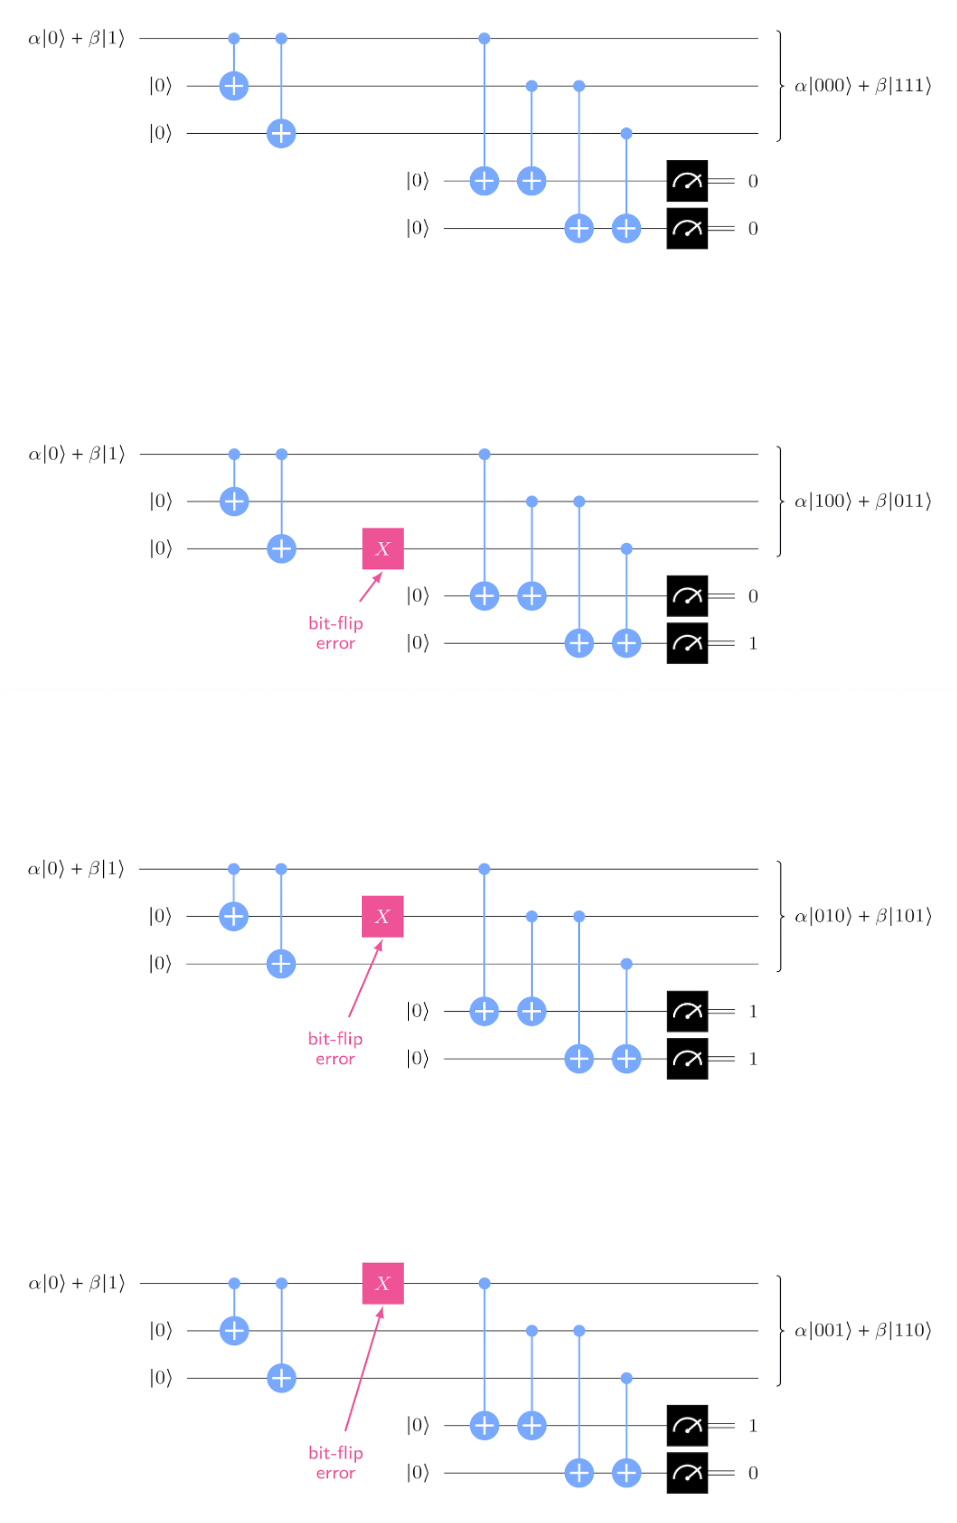
\includegraphics[width=0.75\linewidth]{../images/possbitflip.png}
    \caption{Possible Bit-Flip error circuits}
    \label{fig:possbitflip}
\end{figure}
Crucially, the state of the top three qubits does not collapse in any of the cases, which allows us to correct a bit-flip error if one has occurred - by simply applying it again. The following table \ref{tab:onebitflip} summarizes the states we obtain from at most one bit flip, the measurement outcomes (which are called the syndrome in the context of error correction), and the correction needed to get back to the original encoding.

\begin{table}
    \centering
    \begin{tabular}{|c|c|c|}
    \hline
        State &  Syndrome & Correction \\
        \hline
         $\alpha\ket{000}+\beta\ket{111}$&$00$  &$I\otimes I\otimes I$ \\
         \hline
         $\alpha\ket{100}+\beta\ket{011}$ & $10$   & $X\otimes I\otimes I$\\
         \hline
         $\alpha\ket{010}+\beta\ket{101}$& $11$ & $I\otimes X\otimes I$\\
         \hline
         $\alpha\ket{001}+\beta\ket{110}$&$01$  &$I\otimes I\otimes X$ \\
         \hline
    \end{tabular}
    \caption{One bit-flip error correction}
    \label{tab:onebitflip}
\end{table}
Once again, we're only considering the possibility that at most one bit-flip occurred. this wouldn't work correctly if two or three bit-flips occurred and we also haven't considered other possible errors besides bit-flips.

\section{Phase-flip errors}
In the quantum setting, bit flip errors aren't the only errors we need to worry about. For instance, we also have to worry about phase-flip errors, which are described by $Z$ gates. Along the same lines as bit-flip errors, we can think about phase-flip errors as representing just another possibility of an error that can affect a qubit. However, as we will see in the discretization of errors for quantum error correcting codes, a focus on bit-flip errors and phase-flip errors turns out to be well-justified. Specifically, the ability to correct a bit-flip error, a phase-flip error, or both of these errors simulataneously automatically implies the ability to correct an arbitrary quantum error on a single qubit.

Unfortunately, the $3$-bit repetition code doesn't protect against phase flips at all. For instance, suppose that a qubit state $\alpha\ket{0}+\beta\ket{1}$ has been encoded using the $3$-bit repetition code, and a phase-flip error occurs on the middle qubit. This results in the state
\[
(I\otimes Z\otimes I)(\alpha\ket{000}+\beta\ket{111})=\alpha\ket{000}-\beta\ket{111}
\]
which is exactly the state we would have obtained from encoding the qubit state $\alpha\ket{0}-\beta\ket{1}$. Indeed, a phase-flip error on any one of the three qubits of the encoding has this same effect, which is equivalent to a phase-flip error occurring on the original qubit prior to the encoding. Under the assumption that original quantum state is an unknown state, there's therefore no way to detect that an error has occurred - because it's a perfectly valid encoding of a different qubit state. In particular, running the error detection circuit from before on the state $\alpha\ket{000}-\beta\ket{111}$ is certain to result in the syndrome $00$, which wrongly suggests that no errors have occurred.

Meanwhile, there are now three qubits rather than one that could potentially experience phase-flip errors. So, in a situation in which phase-flip errors are assumed to occur independently on each qubit with some nonzero probability $p$ (similarly to a binary symmetric channel except for phase flips rather than bit flips), this code actually increases the likelihood of a phase-flip error after decoding for small values of $p$. In particular, we'll get a phase-flip error on the original qubit after decoding whenever there are an odd numbers of phase-flip errors on the three qubits of the encoding, which happens with probability $3p(1-p)^2+p^3$. This value is larger than $p$ when $0<p<1/2$. so the code increases the probability of a phase-flip error for values of $p$ in this range.

\subsection{Modified repetition code for phase-flip errors}
We've observed that the $3$-bit repetition code is completely oblivious to phase-flip errors, so it doesn't seem to be very helpful for dealing with this sort of error. We can, however, modify the $3$-bit repetition code in a simple way so that it does detect phase flip errors. this modification will render the code oblivious to bit-flip errors - but as we'll see in the next section, we can combine together the $3$-bit repetition code with this modified versions to obtain the Shor code, which can correct against both bit-flip and phase-flip errors.

Here is the modified version of the encoding circuit from earlier in the lesson, which will now be able to detect phase-flip errors. The modification is very simple: we simply apply a Hadamard gate to each qubit after performing the two controlled-NOT gates.

A Hadamard gate transforms a $\ket{0}$ into a $\ket{+}$ state, and a $\ket{1}$ state into a $\ket{-}$ state, so the next effect is that the single qubit state $\alpha\ket{0}+\beta\ket{1}$ is encoded as
\[
\alpha\ket{+++}+\beta\ket{---}
\]
where $\ket{+++}=\ket{+}\otimes \ket{+}\otimes \ket{+}$ and $\ket{---}=\ket{-}\otimes\ket{-}\otimes\ket{-}$.

A phase flip error, or equivalently a $Z$ gate, flips between the state $\ket{+}$ and $\ket{-}$, so this encoding will be useful for detecting (and correcting) phase-flip errors. Specifically, the error-detection circuit from earlier can be modified as follows \ref{fig:phasefliperr}.
\begin{figure}[ht]
    \centering
    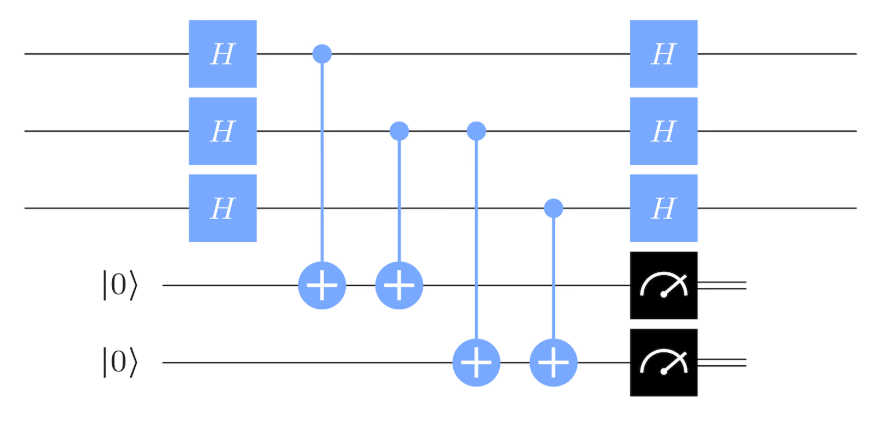
\includegraphics[width=1\linewidth]{../images/phasefliperr.png}
    \caption{Phase-Flip error correction circuit}
    \label{fig:phasefliperr}
\end{figure}
In words, we take the circuit from before and simply put Hadamard gates on the top three qubits at both the beginning and the end. The idea is that the first three Hadamard gate transform $\ket{+}$ and $\ket{-}$ states back into $\ket{0}$ and $\ket{1}$ states, the same parity checks as before takes place, and then the second layer of Hadamard gates transform the states back to $\ket{+}$ and $\ket{-}$ states so that we recover our encoding. For future, reference, let's observe that this phase flip detection circuit can be simplified as follows \ref{fig:phase-fliperr}.
\begin{figure}[ht]
    \centering
    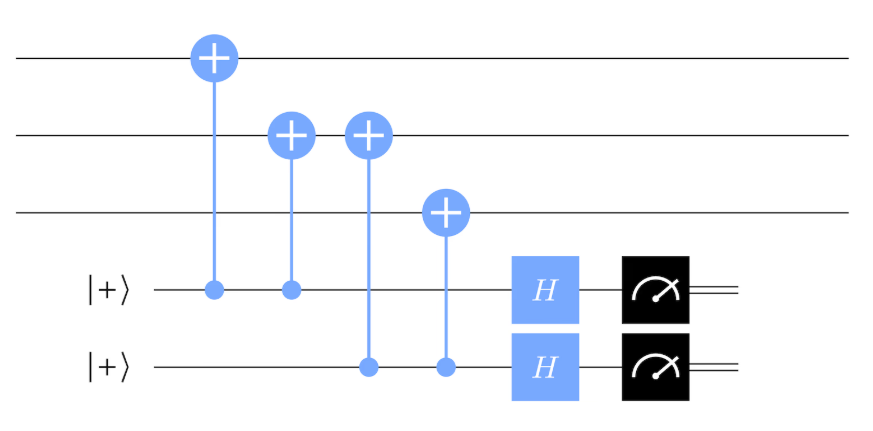
\includegraphics[width=1\linewidth]{../images/phasefliperrorcirc.png}
    \caption{Simplified Phase-Flip correction circuit}
    \label{fig:phase-fliperr}
\end{figure}
The following four circuit diagram \ref{fig:possphaseflip} describe how our modified version of the $3$-bit repetition code, including the encoding step and the error detection step, functions when at most one phase-flip error occurs. The behavior is similar to the ordinary $3$-bit repetition code for bit-flips.
\begin{figure}[ht]
    \centering
    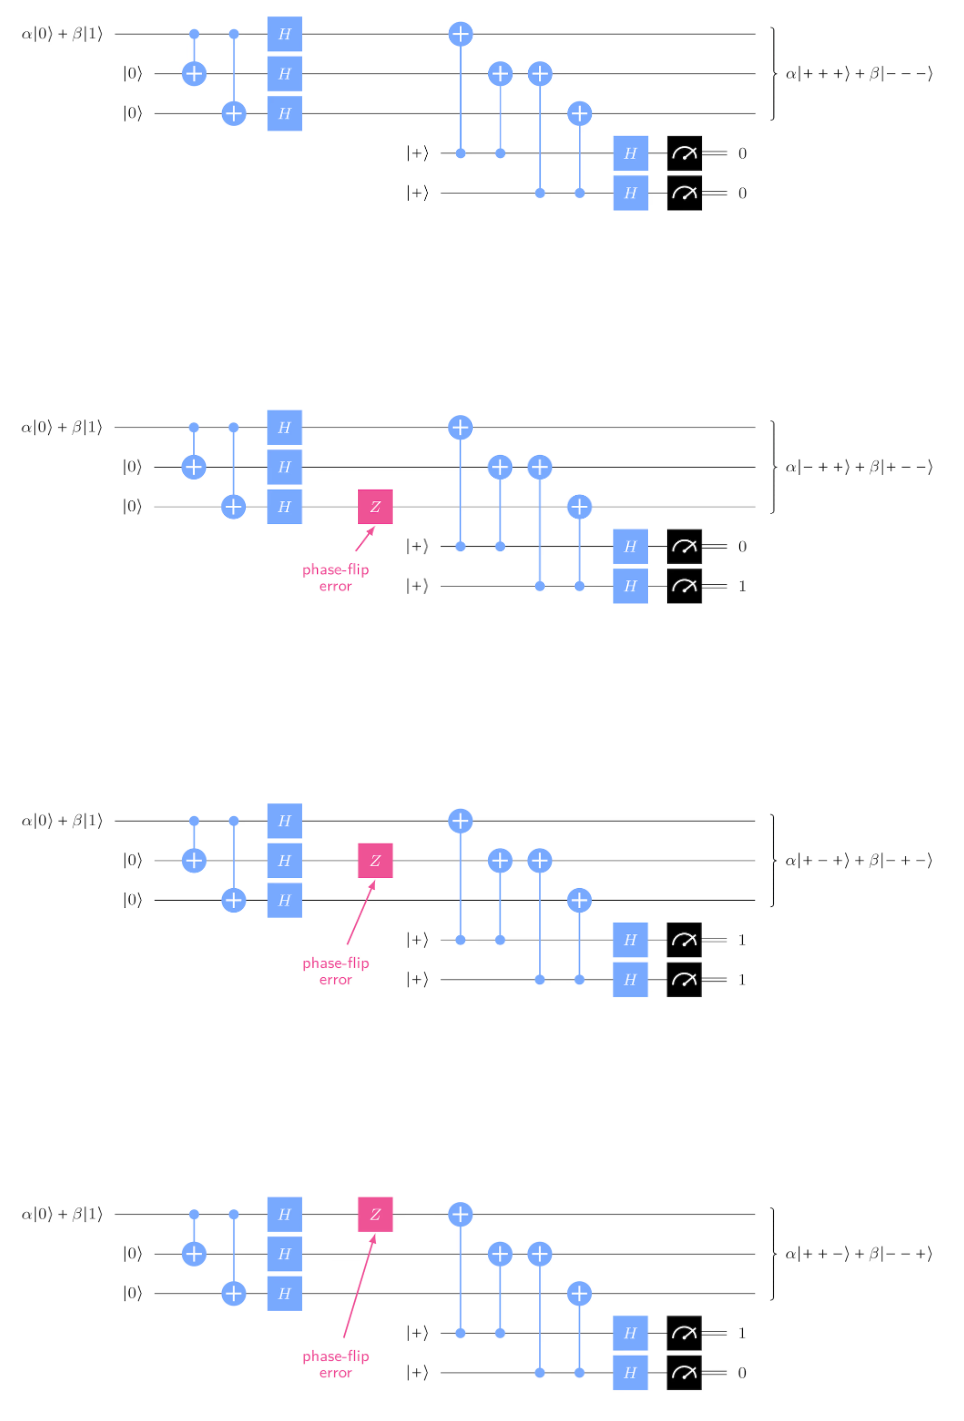
\includegraphics[width=0.75\linewidth]{../images/phasefliperr4circs.png}
    \caption{Possible Phase-Flip error circuits}
    \label{fig:possphaseflip}
\end{figure}
Here's an analogous table to the one from above \ref{tab:phasefliperror}, this time considering the possibility at most one phase-flip error.

\begin{table}[ht]
    \centering
    \begin{tabular}{|c|c|c|}
    \hline
State         & Syndrome & Correction \\
\hline
        $\alpha\ket{+++}+\beta\ket{---}$ & $00$ & $I\otimes I\otimes I$ \\
        \hline
       $\alpha\ket{-++}+\beta\ket{+--}$  & $10$ & $Z\otimes I\otimes I$\\
       \hline
       $\alpha\ket{+-+}+\beta\ket{-+-}$  & $11$ & $I\otimes Z\otimes I$ \\
       \hline
$\alpha\ket{++-}+\beta\ket{--+}$         & $01$  & $I\otimes I\otimes Z$ \\
\hline
    \end{tabular}
    \caption{Phase - flip error correction}
    \label{tab:phasefliperror}
\end{table}
Unfortunately, this modified version of the $3$-bit repetition code can no no longer correct bit-flip errors. Al is not lost, however. As suggested previously, we'll be able to combine these two codes into one code - the $9$-qubit Shor code - that can correct both bit-flip and phase-flip errors (and therefore any error on a single qubit).

\section{The 9-qubit Shor code}
Now we turn to the $9$-qubit Shor code, which is a quantum error correcting code obtained by combining together the two codes considered in the previous section: the $3$-bit repetition code for qubits, which allows for the correction of a single-bit flip error, and the modified version of that code, which allows for the correction of a single phase-flip error.
\subsection{Code description}
To be precise, the $9$-qubit Shor code is the code we obtain by concatenating the two codes from the previous sections. This means that we first apply the other encoding to each of the three qubits used for the first encoding, resulting in $9$ qubits in total. While we could apply the two codes in either order in this particular case, we'll make an arbitrary choice to first apply the modified version of the $3$-bit repetition code (which detect phase-flip errors), and then we'll encode each of the resulting three qubits independently using the original $3$-bit repetition code (which detects bit-flip errors).
Here's a circuit diagram representation of this encoding \ref{fig:9qubitshorcode}.

\begin{figure}[ht]
    \centering
    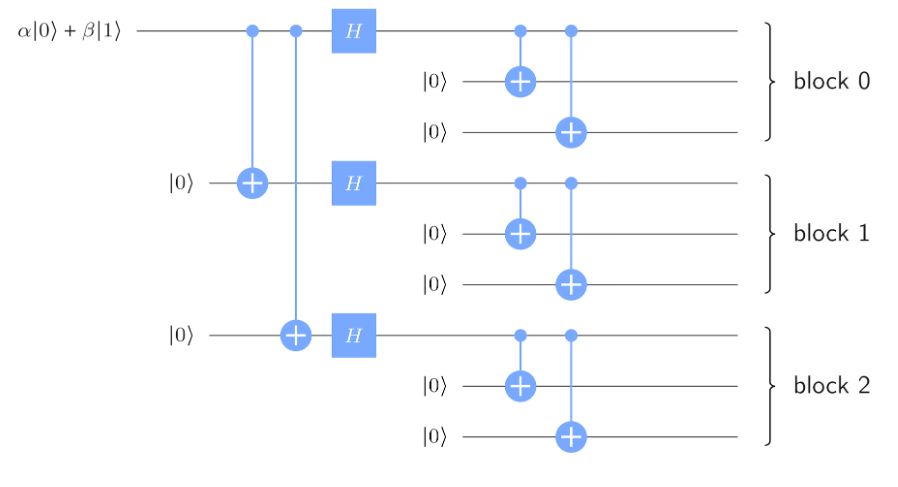
\includegraphics[width=1\linewidth]{../images/9qubitshorcode.png}
    \caption{Circuit Diagram of 9-qubit Shor code}
    \label{fig:9qubitshorcode}
\end{figure}
As the figure suggest, we'll think about the $9$ qubits of the Shor code as being grouped into three blocks of three qubits, where each block is obtained from the second encoding step (which is the ordinary $3$-bit repetition code). The ordinary $3$-bit repetition code, which here is applied three times independently, is called the inner code in the context, whereas the outer code is the code used for the first encoding step, which is the modified version of the $3$-bit repetition code that detects phase-flip errors.

\backmatter  % Use letter page numbering style (A, B, C, D...) for the post-content pages
  % The references (bibliography) information are stored in the file named "references.bib"
    \bibliographystyle{plain}
    \bibliography{references}
\end{document}